
\documentclass[theme=default]{beamer}
\usepackage{graphics}
\usepackage{subfig}
\usepackage{float}
\usepackage{hyperref}
\hypersetup{
    colorlinks = true,
    linkcolor= blue,
    linkbordercolor = {white}
}
\title{BEF: Debt}
\author{Pierre-Carl Michaud}

  \renewcommand*{\thesubfigure}{}
\captionsetup[subfigure]{labelformat=simple}

\begin{document}
\maketitle



\begin{frame}{Household Debt}
\begin{figure}
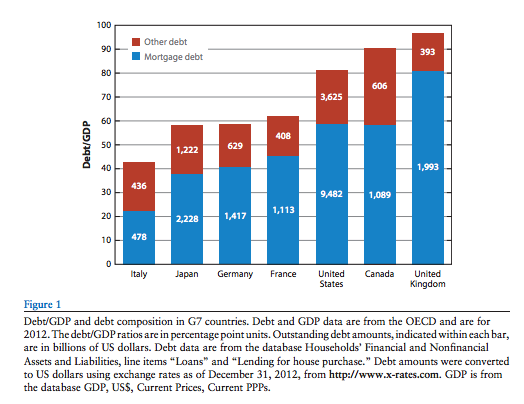
\includegraphics[scale=0.5]{ZinmanDebt.png}
\caption{Zinman (2015)}
\end{figure}
\end{frame}

\begin{frame}{The Rise of Household Debt}
\begin{figure}
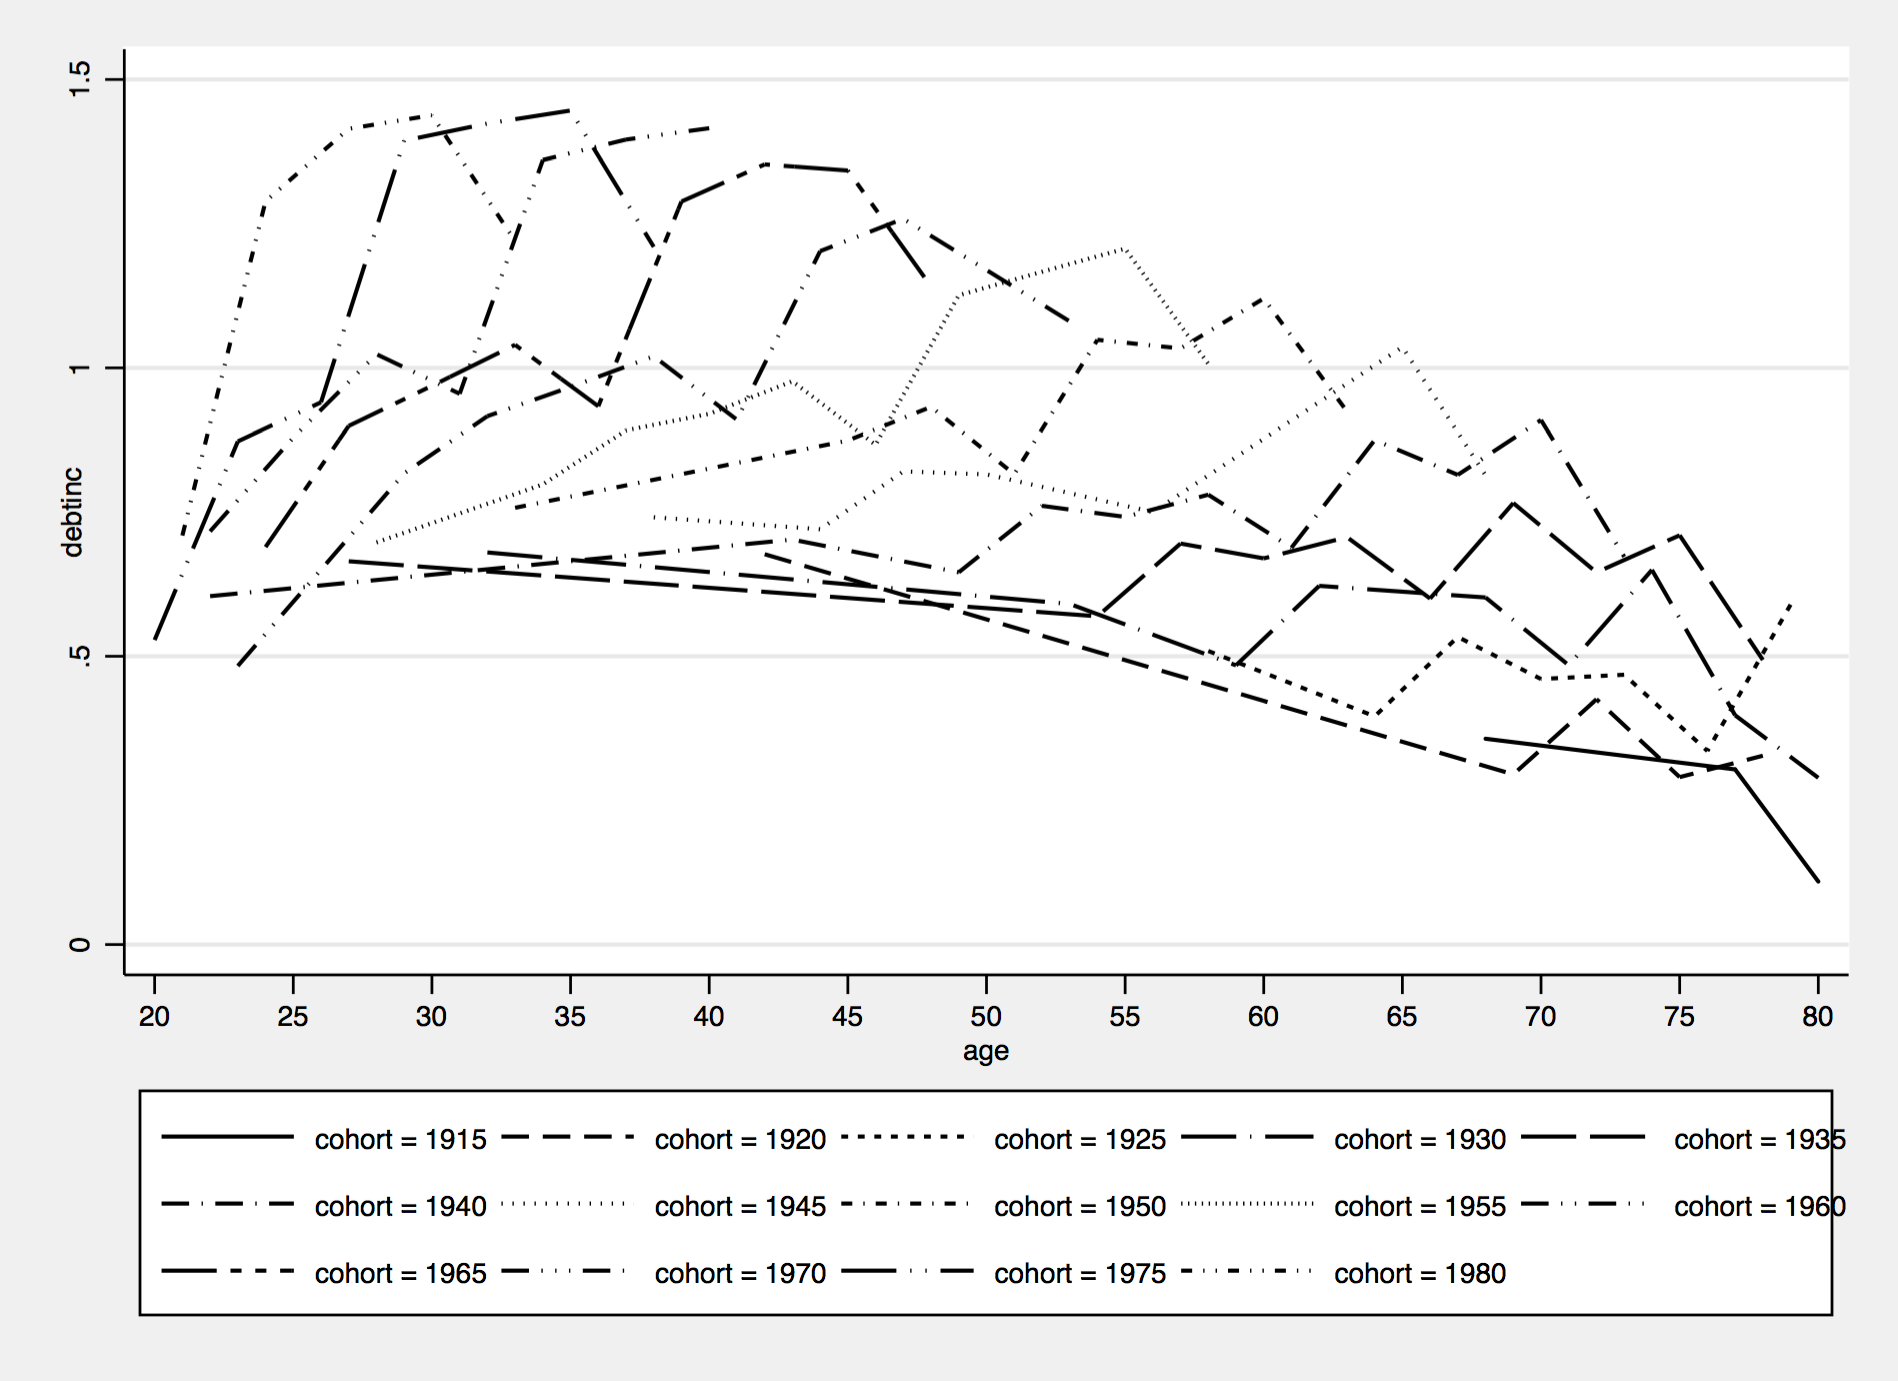
\includegraphics[scale=0.25]{profiles_debtinc.png}
\caption{Own Calculations from SCF. Debt from all sources divided by household income. Is this a good of bad thing? }
\end{figure}
\end{frame}

\begin{frame}{Credit Card Debt}
\begin{figure}
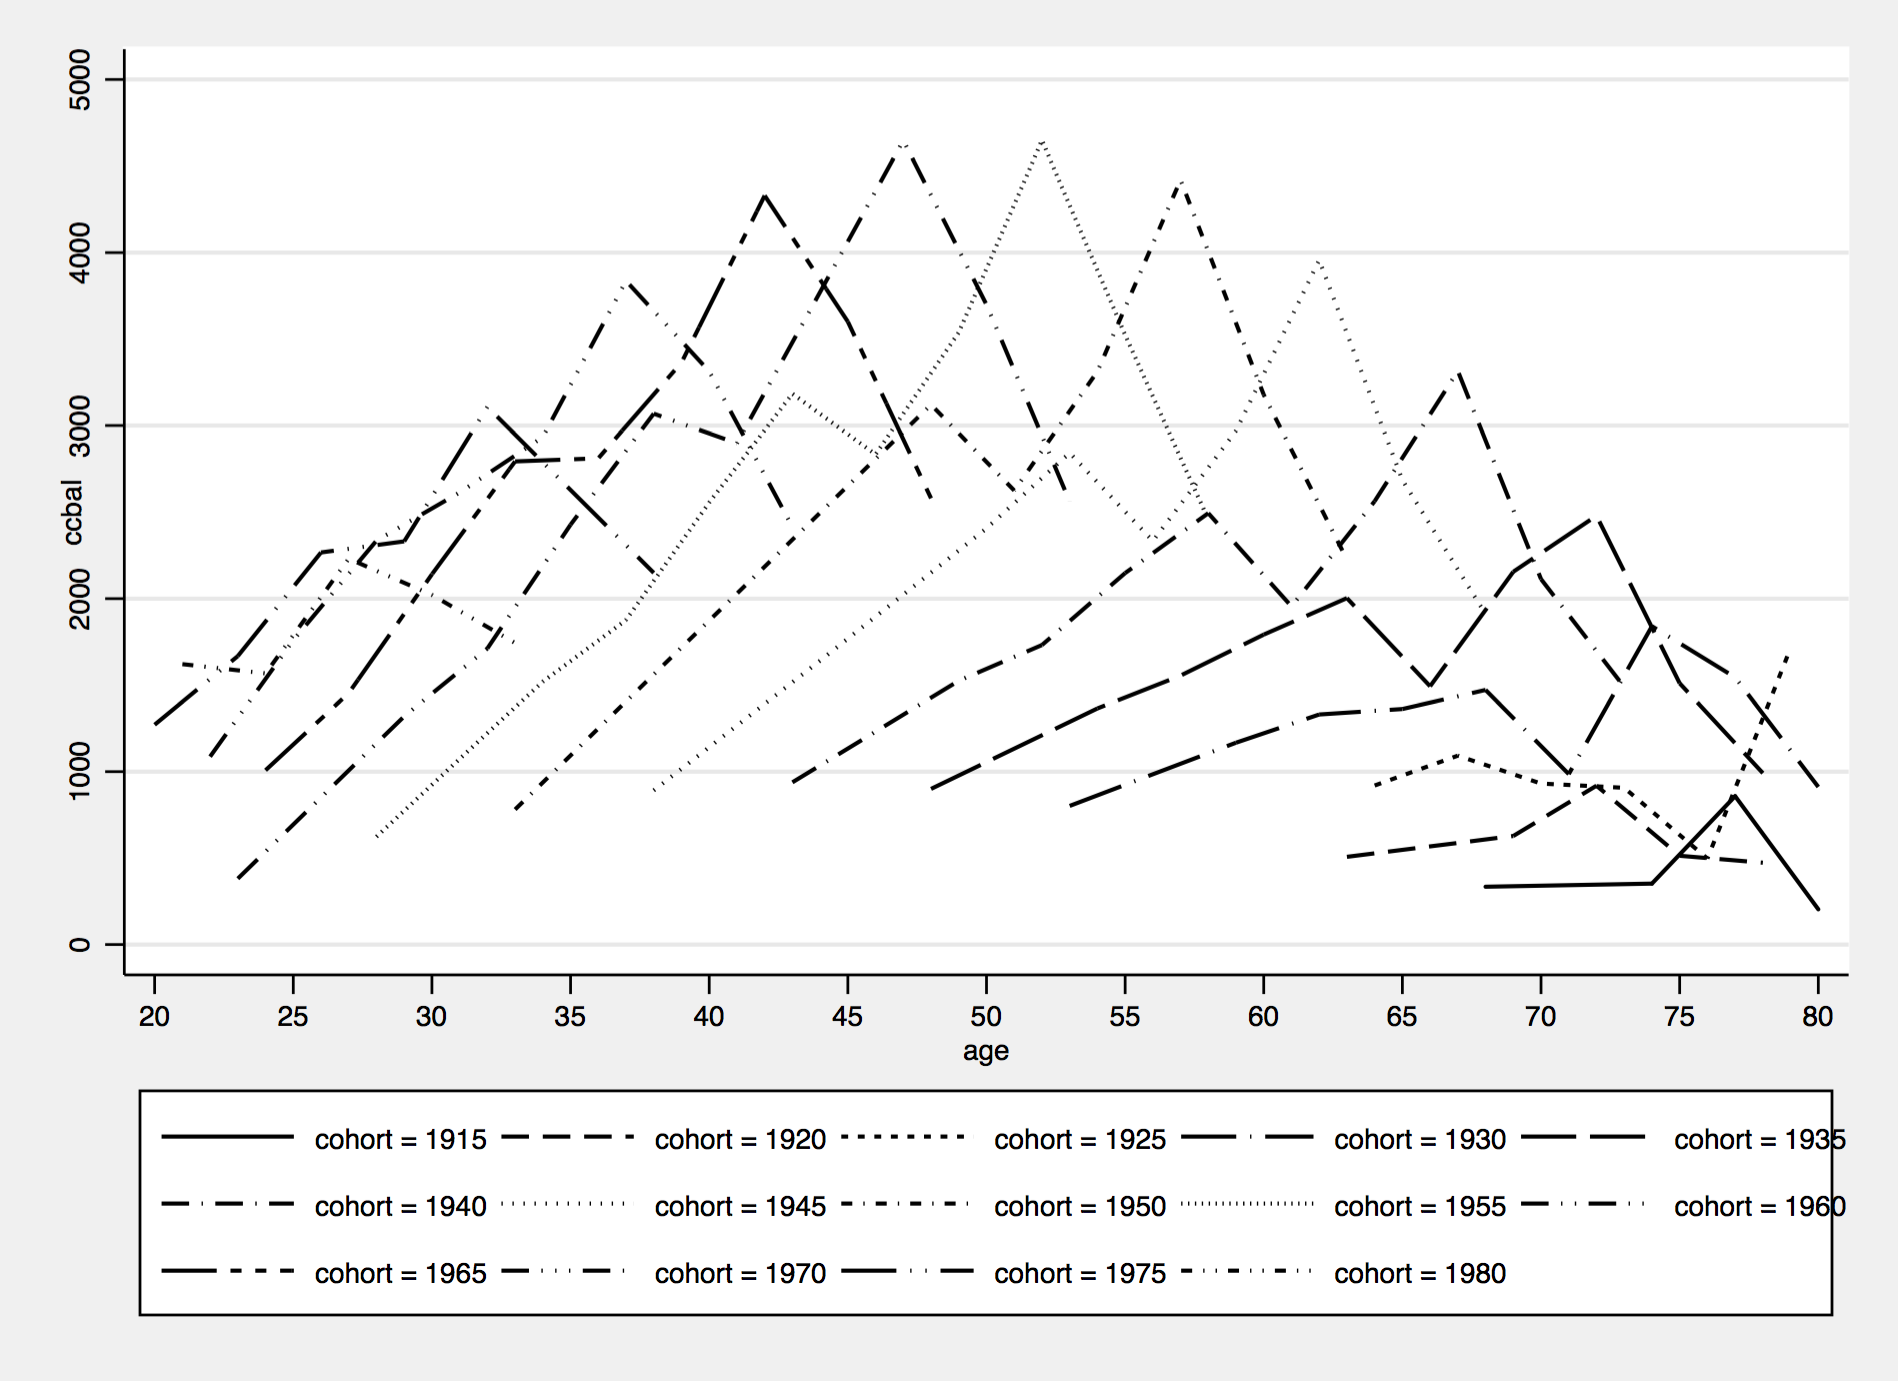
\includegraphics[scale=0.25]{profiles_ccbal.png}
\caption{Own Calculations from SCF. Credit card balances (all cards). 2016 dollars. Financial innovations important?}
\end{figure}
\end{frame}

\begin{frame}{Credit Cards}
\begin{table}[htbp]
\centering
\footnotesize
\input{ccards.tex}
\caption{Statistics on credit card debt held by those age 51-61 in SCF for various years. Weighted using sampling weights provided in SCF. Own calculations. Huge variation in APRs.}
\end{table}

\end{frame}

\begin{frame}{The Literature}
From Zinman (2015):
\begin{itemize}
\item Households borrow more than non-financial companies do (13 trillion compared to 10 trillion)
\item More people have credit cards than participate in the stock market (65 vs. 50\%)
\item Research lags behind considerably relative to asset side of balance sheet
\item We should care because affects poor more, prompt to behavioral biases
\item Example: The Credit card puzzle: no models match prominent use of credit cards as means of financing consumption. 
\end{itemize}
\end{frame}

\begin{frame}{Financing Consumption}

The marginal opportunity cost of financing consumption for various households
\begin{figure}
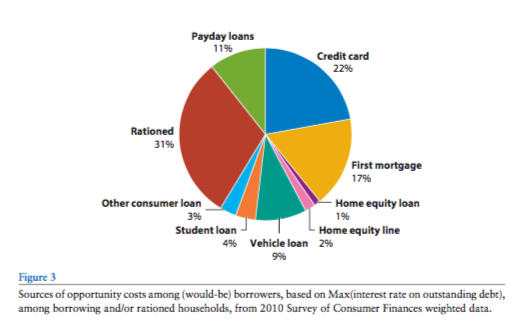
\includegraphics[scale=0.5]{OpportunityCost.png}
\caption{Zinman (2015) }
\end{figure}
\end{frame}


\begin{frame}{Three papers}

Will focus on credit cards and installment loans. Large literature on mortgages (see Zinman (2015) for references). 

Check \href{http://www.nber.org/papers/w24881}{this one for W2019}

\begin{itemize}
\item Agarwal et al. (2015): \textit{Do Consumers Choose the Right Credit Contract?}
\item Stango and Zinman (2011): \textit{Fuzzy Math, Disclosure Regulation and Market Outcomes: Evidence from Truth-in-Lending Reform}
\item Keys and Wang (2016): \textit{Minimum Payments and Debt Paydown in Consumer Credit Cards}

\end{itemize}

\end{frame}

\begin{frame}{Picking the Right Card}

Agarwal et al. (2015)

Questions: 
\begin{itemize}
\item Is the question positive or normative?
\item What type of methodology is used to answer the question?
\item What is the key point the authors make?
\item Does the paper to suffer from limitations? And how did the authors try to adress them?
\end{itemize}


\end{frame}


\begin{frame}{Fuzzy Math and Reform}

Stango and Zinman (2011)

Questions: 
\begin{itemize}
\item Is the question positive or normative?
\item What type of methodology is used to answer the question?
\item What is the key point the authors make?
\item Does the paper to suffer from limitations? And how did the authors try to adress them?
\end{itemize}

\end{frame}


\begin{frame}{Wrapping Up}
From Zinman (2015)
\begin{itemize}
	\item Households do a better job of using existing credit (ex post) than picking the right credit (ex ante)
	\item Welfare effects of financial innovation in credit unclear
	\item Several behavioral biases appear to justify regulation, in particular regarding information
	\item Why is there no financial advice for debt (as we have to investments)?
\end{itemize}
\end{frame}

\end{document}


